\subsection{Décomposition de domaine}
Lorsque le problème a résoudre devient trop gros pour être traité sur une seule machine, il est nécessaire d'adapter la méthode de résolution du problème.
%
Dans le cas du GMRES, nous pouvons utiliser la décomposition de domaine comme préconditionneur parallèle.
%
La décomposition de domaine nous permet de répartir les données sur les différentes unités de calcul.
%
Le découpage en domaines se fera à l'aide d'un logiciel de partitionnement, tel que Scotch ou Metis, avec pour objectif un bon équilibrage de charge et une interaction minime entre les domaines.


Pour la simulation de réservoir, les coefficients de la matrice représentent les interactions entre les cellules du réservoir.
%
Donc si nous partitionnons le graphe de connexions entre les cellules, chaque unité de calcul sera en charge d'un ensemble de cellules (Fig.~\ref{fig:domain}).
%
Nous obtenons donc un préconditionneur totalement parallèle et un bon équilibrage de charge aussi bien en terme de volume de donnée que de volume de calcul.
%
Les autres opérations du GMRES peuvent aussi être faites en parallèle moyennant des opérations de synchronisations coûteuses tel que des réductions à la fin de chaque opération.

%   (-_-)   %
\begin{figure}[t!]
  \centering
  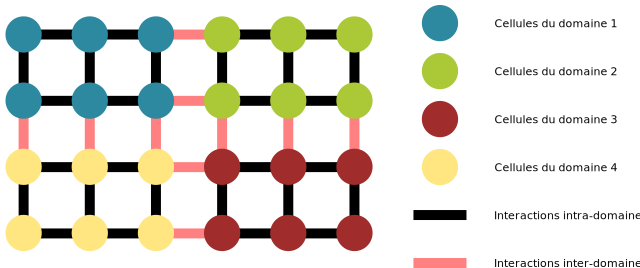
\includegraphics[width=\textwidth]{domain}
  \caption{Décomposition de domaine d'un réservoir à 24 cellules. Il y a deux partitions, chaque partition pouvant être traiter en parallèle.}
  \label{fig:domain}
\end{figure}

En utilisant la méthode de Schwarz additive, ce préconditionneur est totalement parallèle et il ignore les interactions inter-domaines.
%
Malheureusement, plus il y a d'interactions ignorées, moins le préconditionneur est efficace.
%
Formulé différemment, le nombre de domaines aura un impact la convergence du GMRES.
%
C'est pourquoi nous allons essayer de réduire au minimum le nombre de domaines.
